\section{Classification Models}
In this project, various classification techniques were used to identify the most suitable approach. Seven classifiers were applied throughout the Knime workflow, categorized into the following 4 groups:
%\bigskip
\begin{itemize}
    \item \textbf{Heuristic Models}: In this project, Decision Tree (J48), k-Nearest Neighbor (kNN), Random Forest and XGBoost (specific implementation of Gradient Boosting) are applied.
    \item \textbf{Regression based Models}: Logistic regression is used, which models a linear relationship between inputs and a categorical output, using a parametric conditional probability.
    \item \textbf{Separation Models}: Support Vector Machine (Weka's SMO implementation) and Multi-Layer Perceptron are used, which both partition the attributes' space.
    \item \textbf{Probabilistic Models}: Naive Bayes is applied, exploiting Bayes formula and computing posterior probability to classify records.
\end{itemize}

\subsection{Performance Measures}
To evaluate the performance of the models, a variety of measures were computed. These metrics provide a detailed evaluation of classification performance under different conditions. The measures applied are the following:
\begin{itemize}
    \item \textbf{Accuracy}: The number of correct predictions on the total number of predictions. It is calculated as follows:
    \[
    \text{Accuracy} = \frac{TP + TN}{TP + TN + FP + FN}
    \]
    Moreover, it measures the capability of the classification model to give reliable predictions on new records. However, the accuracy measure is not suitable for imbalanced datasets, as in our case. Therefore, the following measures are preferred.

    \item \textbf{Precision}: The fraction of correctly predicted positive records out of all positive predictions. It provides information on the ability of the model to minimize false positives.
    \[
    p = \frac{TP}{TP + FP}
    \]
    \item \textbf{Recall}: The fraction of actual positive records correctly identified by the model. It provides information on the ability of the model to minimize false negatives.
    \[
    r = \frac{TP}{TP + FN}
    \]
    
\end{itemize}

\begin{itemize}
    \item $F_1$ \textbf{measure}: Combines precision ($p$) and recall ($r$) into a single metric by calculating their harmonic mean:
    \[
    F_{measure} = \frac{2 \cdot r \cdot p}{r + p}
    \]
    \item \textbf{ROC and AUC}: The Receiver Operating Characteristic (ROC) curve plots the True Positive Rate (TPR) against the False Positive Rate (FPR) at various classification thresholds. The ROC curve depicts the performance of a classifier without regard to class distribution. Thus, it is useful for confronting different classification models, considering the Area Under the Curve (AUC) value. It ranges from 0 to 1 and measures the overall performance of the classifier. The closer it is to 1, the closer the classifier has TPR to 1 (ideal classifier).
        \begin{figure}[H]
            \centering
            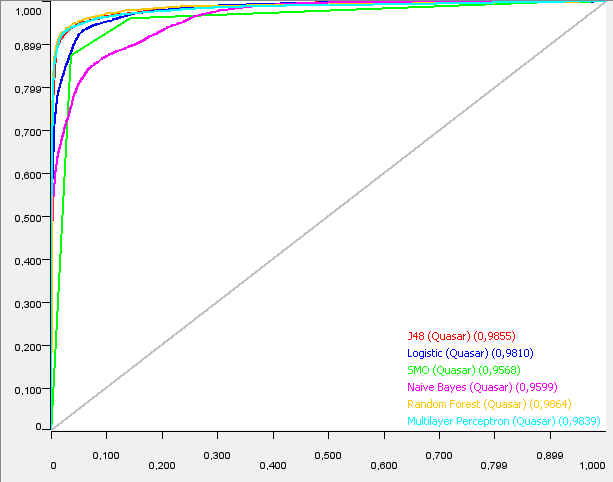
\includegraphics[width=0.9\columnwidth]{images/ROC Quasar MultiClass KFold.png}
            \caption{ROC of Quasar class (initially the least occurrent label) for balanced data from the MultiClassClassifier node.}
            \label{fig:roc_qso_multiclass_kfold}
        \end{figure}
\end{itemize}